\documentclass[aspectratio=169,12pt]{beamer}
\usepackage{amsmath}
\usepackage{amssymb}
\usepackage{xcolor}
\usepackage[most]{tcolorbox}
\usepackage{graphicx}
\usepackage[sfdefault,lf]{FiraSans}
\renewcommand{\familydefault}{\sfdefault}
\setlength{\parindent}{0pt}
\everymath{\displaystyle}

\setbeamertemplate{navigation symbols}{}
\setbeamertemplate{footline}{}
\setbeamertemplate{headline}{}

\definecolor{mmpageWhite}{HTML}{FCFBF7}
\definecolor{mmtanSoft}{HTML}{F7F5EF}
\definecolor{mmgreenDeep}{HTML}{244B2C}
\definecolor{mmgreenLeaf}{HTML}{5D8A56}
\definecolor{mmtext}{HTML}{163221}
\definecolor{mmanswerColor}{HTML}{306A3A}

\setbeamercolor{background canvas}{bg=mmpageWhite}
\setbeamercolor{normal text}{fg=mmtext,bg=mmpageWhite}

\newtcolorbox{MMProblemCard}[1][]{enhanced,breakable=false,colback=white,colframe=black,boxrule=1.0pt,arc=5pt,left=3pt,right=3pt,top=2pt,bottom=2pt,before skip=0pt,after skip=0pt,height=0.22\textheight,valign=top,#1}
\newcommand{\KoruIcon}{\raisebox{-0.2em}{
\includegraphics[height=1.05em]{img/header-logo.png}}}
\newcommand{\HoeIcon}{\raisebox{-0.2em}{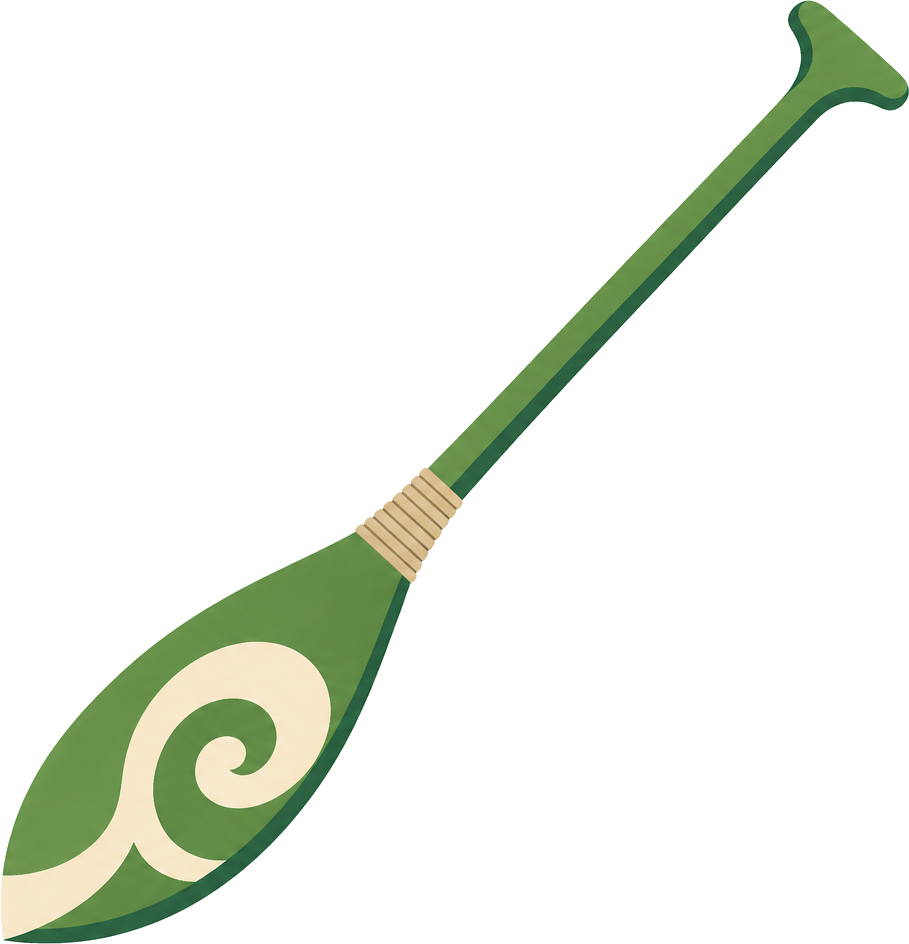
\includegraphics[height=1.05em]{img/hoe.png}}}
\newcommand{\ScaffoldIcons}[1]{\ifcase#1\or \HoeIcon\or \HoeIcon\hspace{0.22em}\HoeIcon\or \HoeIcon\hspace{0.22em}\HoeIcon\hspace{0.22em}\HoeIcon\fi}
\newcommand{\WorksheetTitle}[2]{
  \colorbox{mmtanSoft}{\parbox[c][2.0em][c]{0.975\linewidth}{\hspace{0.25em}{\Large\bfseries\textcolor{mmgreenDeep}{#1}\hfill\ScaffoldIcons{#2}}}}
  \par\vspace{0.08em}{\color{mmgreenLeaf}\rule{\linewidth}{2.0pt}}\par\vspace{0.04em}}
\newcommand{\MMAnswer}[2]{\begin{MMProblemCard}\raggedright\small\textbf{#1.} \textcolor{mmanswerColor}{\textbf{#2}}\par\end{MMProblemCard}}

\setbeamertemplate{background}{\begin{tikzpicture}[remember picture,overlay]\draw[black,line width=1.5pt,rounded corners=10pt]([xshift=0.45cm,yshift=-0.45cm]current page.north west) rectangle ([xshift=-0.45cm,yshift=0.45cm]current page.south east);\end{tikzpicture}}

\begin{document}
\begin{frame}[t]
\WorksheetTitle{Build Tasks - Answers}{2}
\vspace{-0.18em}
\begin{columns}[T,onlytextwidth]
\begin{column}{0.32\textwidth}\MMAnswer{1}{37°}\end{column}
\begin{column}{0.32\textwidth}\MMAnswer{2}{82°}\end{column}
\begin{column}{0.32\textwidth}\MMAnswer{3}{127°}\end{column}
\end{columns}
\vspace{0.45em}
\begin{columns}[T,onlytextwidth]
\begin{column}{0.32\textwidth}\MMAnswer{4}{23°}\end{column}
\begin{column}{0.32\textwidth}\MMAnswer{5}{148°}\end{column}
\begin{column}{0.32\textwidth}\MMAnswer{6}{66°}\end{column}
\end{columns}
\vspace{0.45em}
\begin{columns}[T,onlytextwidth]
\begin{column}{0.32\textwidth}\MMAnswer{7}{99°}\end{column}
\begin{column}{0.32\textwidth}\MMAnswer{8}{42°}\end{column}
\begin{column}{0.32\textwidth}\MMAnswer{9}{155°}\end{column}
\end{columns}
\end{frame}
\begin{frame}[t]
\WorksheetTitle{Build Tasks - Answers}{2}
\vspace{-0.18em}
\begin{columns}[T,onlytextwidth]
\begin{column}{0.32\textwidth}\MMAnswer{10}{Estimate varies; actual 35°. Error = |estimate - 35|}\end{column}
\begin{column}{0.32\textwidth}\MMAnswer{11}{Estimate varies; actual 70°. Error = |estimate - 70|}\end{column}
\begin{column}{0.32\textwidth}\MMAnswer{12}{Estimate varies; actual 115°. Error = |estimate - 115|}\end{column}
\end{columns}
\vspace{0.45em}
\begin{columns}[T,onlytextwidth]
\begin{column}{0.32\textwidth}\MMAnswer{13}{Estimate varies; actual 50°.}\end{column}
\begin{column}{0.32\textwidth}\MMAnswer{14}{Estimate varies; actual 130°.}\end{column}
\begin{column}{0.32\textwidth}\MMAnswer{15}{Estimate varies; actual 85°.}\end{column}
\end{columns}
\vspace{0.45em}
\begin{columns}[T,onlytextwidth]
\begin{column}{0.32\textwidth}\MMAnswer{16}{C (more than 180°)}\end{column}
\begin{column}{0.32\textwidth}\MMAnswer{17}{C (obtuse)}\end{column}
\begin{column}{0.32\textwidth}\MMAnswer{18}{D (reflex)}\end{column}
\end{columns}
\end{frame}
\begin{frame}[t]
\WorksheetTitle{Build Tasks - Answers}{2}
\vspace{-0.18em}
\begin{columns}[T,onlytextwidth]
\begin{column}{0.32\textwidth}\MMAnswer{19}{Reflex = 360° - 145° = 215°}\end{column}
\begin{column}{0.32\textwidth}\MMAnswer{20}{Reflex = 360° - 55° = 305°}\end{column}
\begin{column}{0.32\textwidth}\MMAnswer{21}{Reflex = 360° - 120° = 240°}\end{column}
\end{columns}
\vspace{0.45em}
\begin{columns}[T,onlytextwidth]
\begin{column}{0.32\textwidth}\MMAnswer{22}{a) acute, b) obtuse, c) straight, d) reflex}\end{column}
\begin{column}{0.32\textwidth}\MMAnswer{23}{C (Start from 0° on whichever scale lines up)}\end{column}
\begin{column}{0.32\textwidth}\MMAnswer{24}{B (140°)}\end{column}
\end{columns}
\vspace{0.45em}
\begin{columns}[T,onlytextwidth]
\begin{column}{0.32\textwidth}\MMAnswer{25}{78°, acute}\end{column}
\begin{column}{0.32\textwidth}\MMAnswer{26}{33°, acute}\end{column}
\begin{column}{0.32\textwidth}\MMAnswer{27}{163°, obtuse}\end{column}
\end{columns}
\end{frame}
\end{document}
